%\documentclass[9pt, aspectratio=169]{beamer}
\documentclass[9pt, handout, aspectratio=169]{beamer}		% For use when we want to skip \pause commands exporting
\usetheme{PedroRiveroANLwide}

%\setbeameroption{show notes}
%\setbeameroption{show only notes}
\setbeamerfont{note page}{size=\fontsize{0.2cm}{0.1cm}}

%%%%%%%%%%%%%%%%%%%%%%%%%%%%%%%%%%%%%%%%%%%%
%%%%%%%%%%         TITLE          %%%%%%%%%%
%%%%%%%%%%%%%%%%%%%%%%%%%%%%%%%%%%%%%%%%%%%%

\title{Quantum Computing of the Deuteron Binding Energy}
\subtitle{Improving on \href{https://arxiv.org/abs/1801.03897}{arXiv:1801.03897}}
\author{Pedro Rivero}
\newcommand{\mail}{priveroramirez@anl.gov}
\date{\emph{\small{\today}}}
\institute{Argonne National Laboratory\\ Illinois Institute of Technology\\
\href{mailto:\mail}{\nolinkurl{\mail}}}
\newcommand{\website}{www.phy.anl.gov}

\begin{document}
\justify
\setlength{\abovedisplayskip}{0pt}
\setlength{\belowdisplayskip}{12pt}
\setlength{\abovedisplayshortskip}{0pt}
\setlength{\belowdisplayshortskip}{12pt}

	\begin{frame}[plain,t]
		\titlepage
	\end{frame}

	\begin{frame}[c]{Contents Overview}
%		\begin{multicols}{2}
%  			\tableofcontents
%		\end{multicols}
		\tableofcontents
	\end{frame}

%%%%%%%%%%%%%%%%%%%%%%%%%%%%%%%%%%%%%%%%%%%%
%%%%%%%%%%          BODY          %%%%%%%%%%
%%%%%%%%%%%%%%%%%%%%%%%%%%%%%%%%%%%%%%%%%%%%

\section{Introduction}

	\begin{frame}{What is Quantum Computing?}

		Quantum Computing is the application of \textbf{Quantum Information Science (QIS)} to the development of \textit{machines} capable of performing operations and calculations based on quantum logic instead of the usual classical logic.

		\medskip

		The usefulness of this kind of computation lays not only on the ability to engineer exponentially faster machines, but also on things such as being able to \textbf{efficiently simulate nature at the quantum level}, or creating encryption systems which are fundamentally secure.

		\medskip

		\begin{multicols}{2}

			\underline{\textbf{CLASSICAL LOGIC}}\\
			Set Theory (Boolean algebra)

			\medskip

			\begin{itemize}
				\item \textbf{AND} $\quad \Rightarrow \quad A \cup B$
				\item \textbf{OR} $\quad \Rightarrow \quad A \cap B$
				\item \textbf{NOT} $\quad \Rightarrow \quad \overline{A}$
				\item \textbf{XOR} $ \quad \Rightarrow \quad A \cap B - A \cup B$
			\end{itemize}

			\columnbreak

			\underline{\textbf{	QUANTUM LOGIC}}\\
			Quantum Theory (Non-Commutative)

			\medskip

			\begin{itemize}
				\item \textbf{Probabilistic measurement}
				\item \textbf{Measurement causes disturbance}
				\item \textbf{Superposition}
				\item \textbf{Entanglement}
				\item \textbf{Uncertainty principle}
			\end{itemize}

		\end{multicols}

	\end{frame}

%%%%%%%%%%%%%%%%%%%%%%%%%%%%%%%%%%%%%%%%%%%%

	\subsection{The Abacus Effect}

	\begin{frame}{The Abacus Effect}

		To try to understand the power of Quantum Computing in abstract, we can resort to what might be called \textbf{"The Abacus Effect"}.

		\medskip

		Before the abacus was invented, the only way of counting was through a "thermometer-like" scale, which was highly inefficient as it meant adding one physical bead per unit. The abacus did something great: it introduced the concept of \textbf{digits}, which was later put into an even more concise notation by the Arabs through the introduction of \textbf{numerals}.

		\medskip

		This means that, instead of counting up to $N$ using $N$ raw elements, we can count using only $\text{log}_b (N)$ abacus elements ---where $b$ is the base of our number system (i.e. the amount of beads per row in the abacus). Therefore, for $b\geq2$, the abacus introduced an \textbf{exponential decrease in resource requirements} to represent the exact same thing.

		\medskip

		Quantum computers do something analogous. To represent the quantum state of a system made out of $N$ subsystems ---each of which with $b$ degrees of freedom--- we would usually need $b^N$ classical elements (i.e. numbers). By using quantum systems for this representation, we would only need $N$ quantum elements (i.e. each subsystem). Again, an exponential decrease in resource requirements.

	\end{frame}

%%%%%%%%%%%%%%%%%%%%%%%%%%%%%%%%%%%%%%%%%%%%

	\subsection{Quantum Software}

	\begin{frame}{Quantum Software: IBM's Qiskit}

		\medskip

		Working with quantum systems is extremely difficult, and in many cases very expensive, this makes quantum computing research unavailable to many groups and institutions. In order to solve this problem, IBM has developed \textbf{Qiskit}, a python framework for quantum computation and quantum information.

		\begin{multicols}{2}

			This framework allows the construction of quantum circuits ---today's most common way of representing quantum computation--- for running using different backends. These backends range from simulators to actual quantum devices accessible on the cloud through the \textbf{IBMQ API}. It also includes tools for handling noise and error correction, developing quantum based applications and tools, or making use of well known, pre-programmed algorithms. On top of that, it allows work at different levels of abstraction.

			\columnbreak

			\begin{center}
				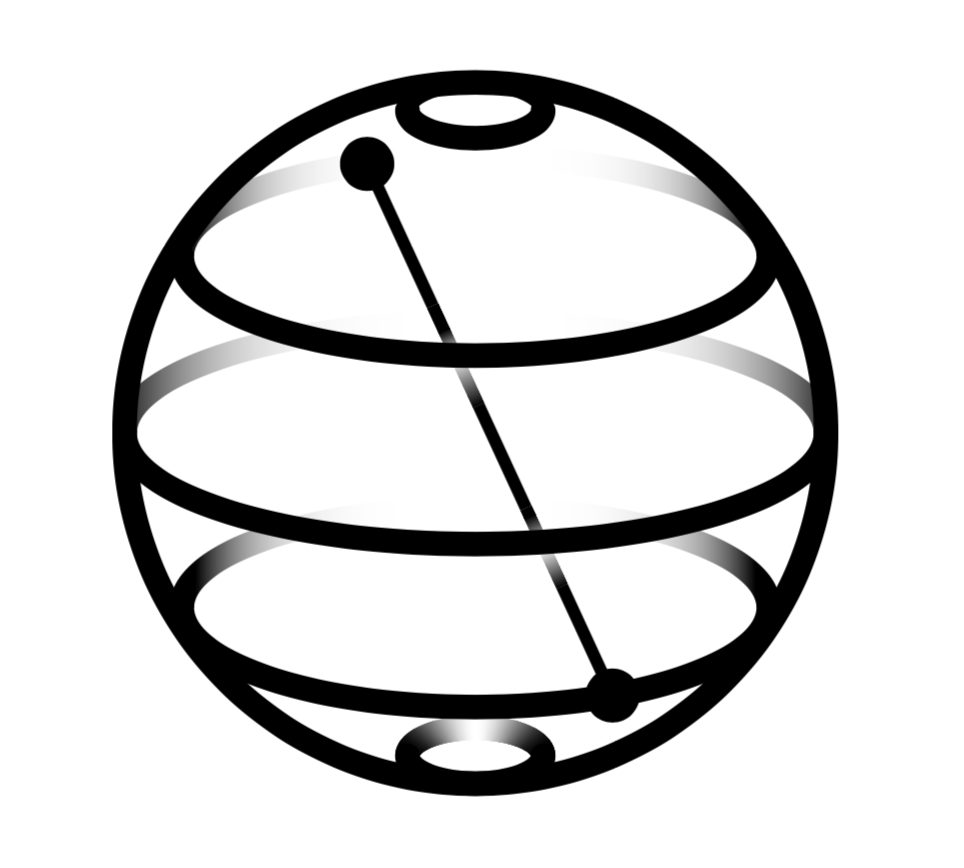
\includegraphics[height=.44\paperheight]{Figures/qiskit}
			\end{center}

		\end{multicols}

	\end{frame}

%%%%%%%%%%%%%%%%%%%%%%%%%%%%%%%%%%%%%%%%%%%%
%%%%%%%%%%%%%%%%%%%%%%%%%%%%%%%%%%%%%%%%%%%%

\section{Case Study}

	\begin{frame}{Case Study}

		As a starting point we decided to reproduce the paper \textbf{Cloud Quantum Computing of an Atomic Nucleus} (\href{https://arxiv.org/abs/1801.03897}{arXiv:1801.03897}) by Dumitrescu \textit{et al.}

		\medskip

		In this paper, IBM's QX5 quantum computer was used to simulate the \textbf{deuteron binding energy}, through a Hamiltonian from pionless effective field theory:

		\begin{align*}
			H_N = \sum^{N-1}_{n,n'=0} \mel{n'}{(T+V)}{n}a^{\dagger}_{n'}a_{n}
		\end{align*}

		Where $N$ is the dimension for a discrete variable representation in the harmonic oscillator basis.

		\begin{gather*}
			\mel{n'}{T}{n} = \frac{\hbar \omega}{2} \left[
				\left( 2n + \frac{3}{2} \right) \delta_n^{n'} -
				\sqrt{ n \left( n + \frac{1}{2} \right) } \delta_n^{n'+1} -
				\sqrt{ \left( n + 1 \right) \left( n + \frac{3}{2} \right) } \delta_n^{n'-1} \right] \\
			\mel{n'}{V}{n} = V_0 \delta_n^0 \delta_n^{n'}
		\end{gather*}

	\end{frame}

%%%%%%%%%%%%%%%%%%%%%%%%%%%%%%%%%%%%%%%%%%%%

	\subsection{Hamiltonian Mapping}

	\begin{frame}{Hamiltonian Mapping onto qubits}

		In order to simulate a quantum system on a quantum computer, we need to map its Hamiltonian onto the qubits of the device. To do so, in this case, we can use the \textbf{Jordan-Wigner transformations} which map the creation/annihilation operators onto Pauli matrices. This is necesarry as no direct measurement of a general quantum operator can be performed in a quanutm computer. However, it is possible to perform Pauli measurements with ease.

		\begin{align*}
			a^{\dagger}_{n} \rightarrow \frac{1}{2} \left[ \prod^{n-1}_{j=0} -Z_j \right] (X_n - i Y_n)
			\hspace{40pt}
			a_{n} \rightarrow \frac{1}{2} \left[ \prod^{n-1}_{j=0} -Z_j \right] (X_n + i Y_n)
		\end{align*}

		Where a spin up $\ket{\uparrow}$ on qubit $n$ represents zero deuteron in state $\ket{n}$, and a spin down $\ket{\downarrow}$ one deuteron. For different values of $N$, this returns:

		\begin{align*}
			H_1 &= 0.218291(Z_0 - I) \quad \Rightarrow \quad E_1 = \mel{\downarrow}{H_1}{\downarrow} \simeq -0.436 \text{MeV} \\
			H_2 &= 5.906709 I + 0.218291 Z_0 - 6.125 Z_1 - 2.143304(X_0 X_1 + Y_0 Y_1) \\
			H_3 &= H_2 + 9.625(I-Z_2) - 3.913119(X_1 X_2 + Y_1 Y_2) \\
			&\cdots
		\end{align*}

		\vspace{-20pt}

	\end{frame}

%%%%%%%%%%%%%%%%%%%%%%%%%%%%%%%%%%%%%%%%%%%%

	\subsection{Unitary Coupled Cluster}

	\begin{frame}{Unitary Coupled Cluster}

		To determine ground-state energy we first need to know the region of Hilbert-space representing valid states of our quantum system. Then, we can use the \textbf{Unitary Coupled Cluster ansatz}. For this, we define unitary operators entangling two and three orbitals:

		\begin{align*}
			U_2(\theta) &= \text{exp} \left[ \theta(a_0^\dagger a_1 - a_1^\dagger a_0) \right] = \text{exp}\left[ i\frac{\theta}{2}(X_0 Y_1 - X_1 Y_0) \right] \\
			U_3(\eta, \theta) &= \text{exp} \left[ \eta(a_0^\dagger a_1 - a_1^\dagger a_0) + \theta(a_0^\dagger a_2 - a_2^\dagger a_0) \right] \\
			&\simeq \text{exp}\left[ i\frac{\eta}{2}(X_0 Y_1 - X_1 Y_0) \right] \text{exp}\left[ i\frac{\theta}{2}(X_0 Z_1 Y_2 - X_2 Z_1 Y_0) \right]
		\end{align*}

		These operators will transform our initial quantum state into some other state in the region of interest according to their parameters.

	\end{frame}

%%%%%%%%%%%%%%%%%%%%%%%%%%%%%%%%%%%%%%%%%%%%

	\subsection{Quantum Circuits}

	\begin{frame}{Quantum Circuits}

		\medskip

		Once we have the unitary operators which get us from an initial state to some other state in the region of interest, we can implement them as \textbf{quantum circuits} and run them through qiskit.

		\begin{multicols}{2}

			\begin{center}
				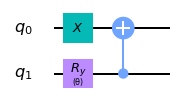
\includegraphics[height=.24\paperheight]{Figures/u2_circuit}
			\end{center}

			\columnbreak

			\begin{center}
				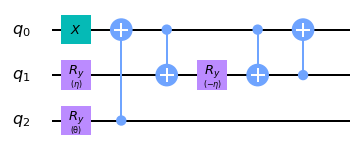
\includegraphics[height=.24\paperheight]{Figures/u3_circuit}
			\end{center}

		\end{multicols}

		These circuits implement the transformations given by the previously introduced unitary operators from the UCC ansatz. Afterwards, the states are \textbf{measured}:

		\begin{multicols}{2}

			\begin{center}
				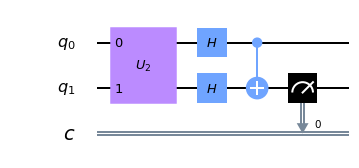
\includegraphics[height=.24\paperheight]{Figures/u2_measure}
			\end{center}

			\columnbreak

			\begin{center}
				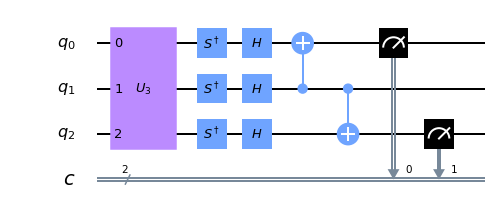
\includegraphics[height=.24\paperheight]{Figures/u3_measure}
			\end{center}

		\end{multicols}

	\end{frame}

%%%%%%%%%%%%%%%%%%%%%%%%%%%%%%%%%%%%%%%%%%%%

	\subsection{VQE Algorithm}

	\begin{frame}{VQE Algorithm}

		Now that we have a possible ground-state, we can obtain the expected value for its energy by performing several Pauli measurements, take the averages, and add them up all otgether according to the weights given by the transformed hamiltonians. This will result in the \textbf{expectation value for the deuteron hamiltonian}, just as we wanted.

		\medskip

		Now we need a way of finding the state which \textbf{minimizes this energy}, which will correspond by definition to the ground-state. To do so, we make use of a quantum-classical hybrid algorithm called \textbf{VQE algorithm}:

		\begin{center}
			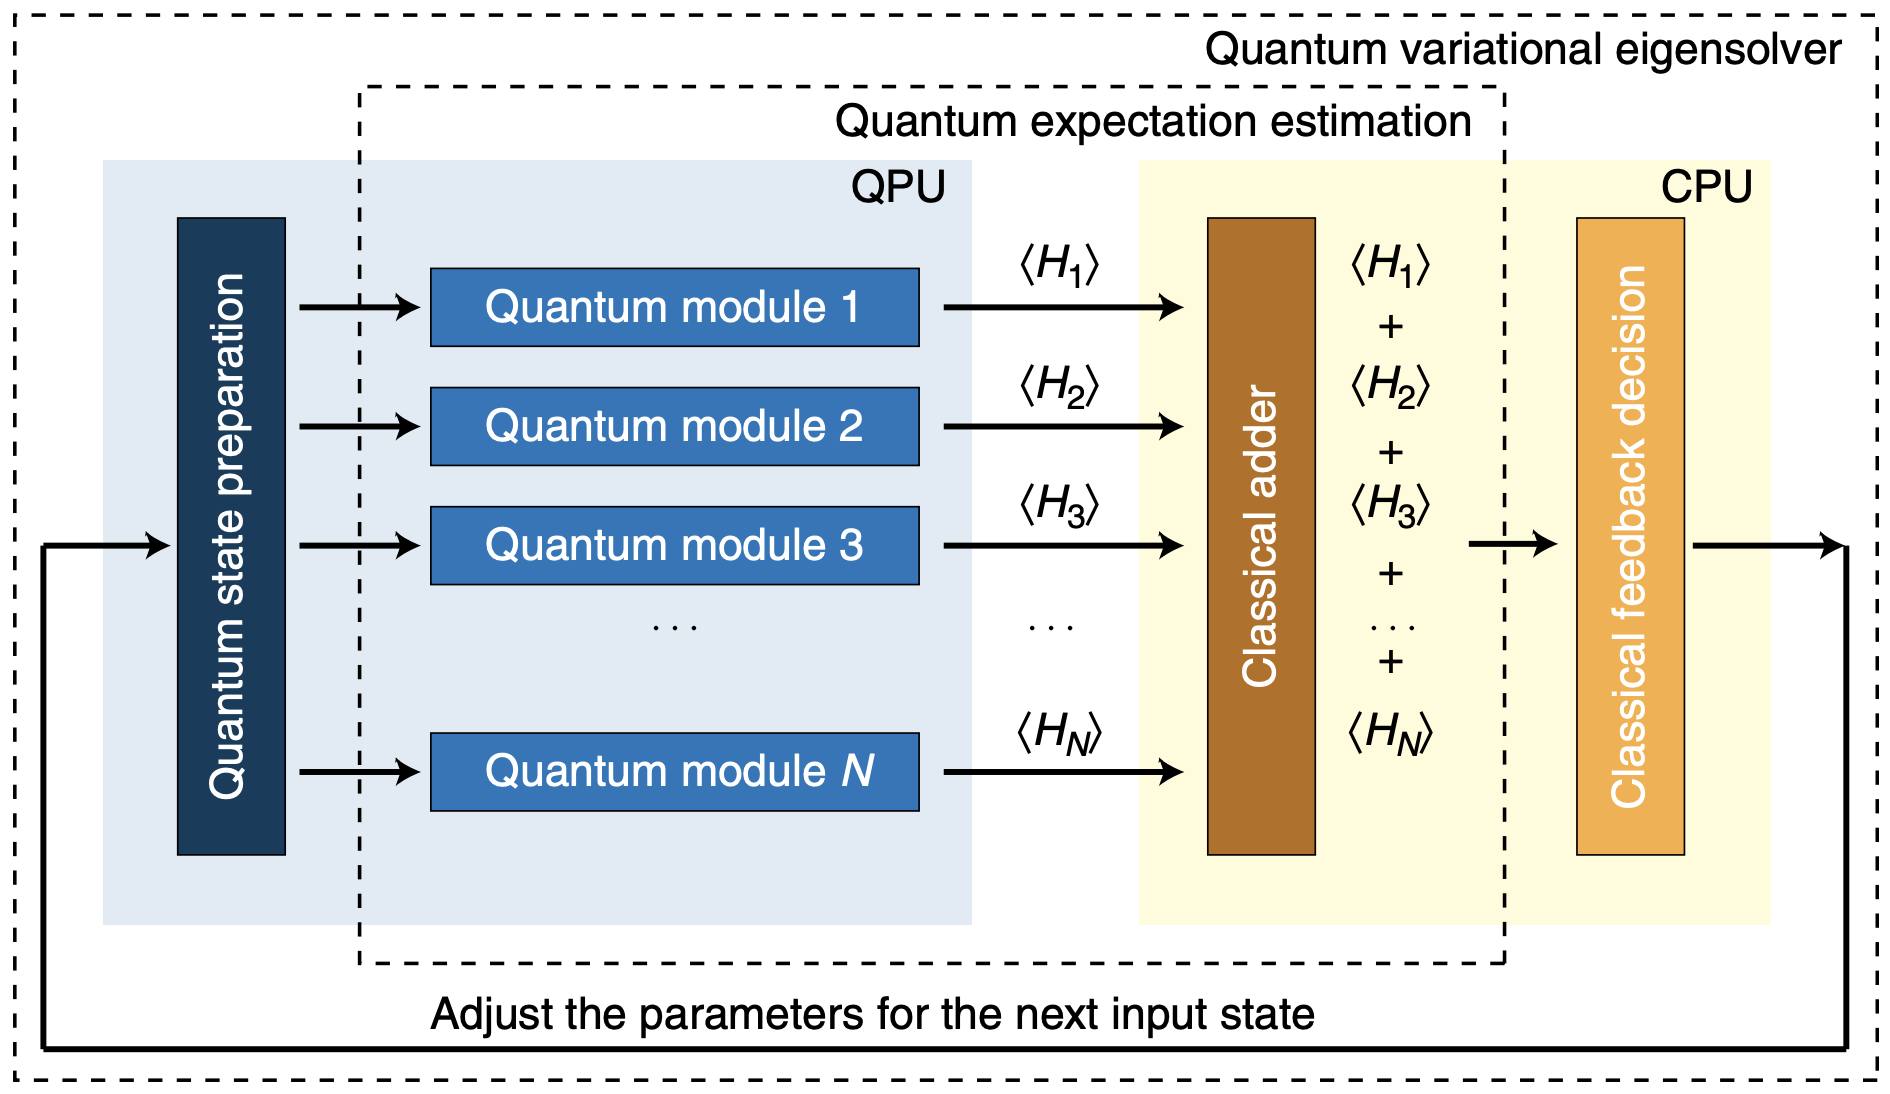
\includegraphics[height=.44\paperheight]{Figures/vqe_algorithm}
		\end{center}

	\end{frame}

%%%%%%%%%%%%%%%%%%%%%%%%%%%%%%%%%%%%%%%%%%%%

	\subsection{Results}

	\begin{frame}{Results for the two Hamiltonians}

		The results we get from this strategy can verify by plotting the expected energy for the entire region of space in both cases:

		\begin{multicols}{2}

			\begin{center}
				\texttt{ \small
					GROUND-STATE ENERGY (H2): \\
					Minimum \underline{'E2 = -1.8100 (MeV)'} \\
					'theta = 0.6202 (rad)' \\
					>> ERROR = 3.5\% } \\
				\smallskip
				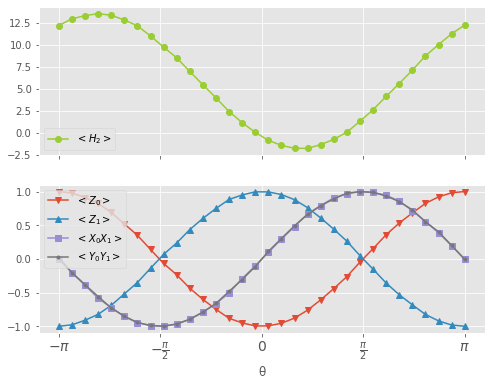
\includegraphics[height=.40\paperheight]{Figures/h2_result}
			\end{center}

			\columnbreak

			\begin{center}
				\texttt{ \small
					GROUND-STATE ENERGY (H3): \\
					Minimum \underline{'E3 = -2.0513 (MeV)'} \\
					'[theta, eta] = [0.2819, 0.3040] (rad)' \\
					>> ERROR = 0.3\% } \\
				\smallskip
				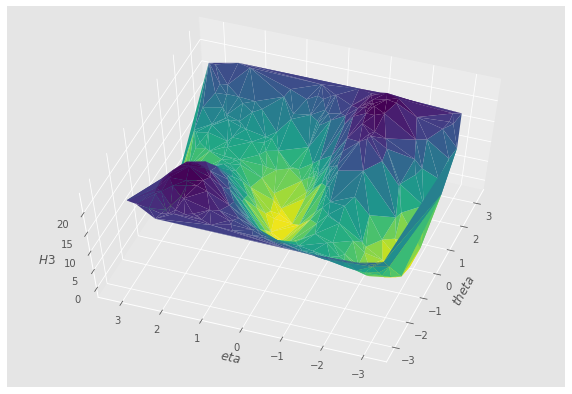
\includegraphics[height=.40\paperheight]{Figures/h3_result}
			\end{center}

		\end{multicols}

	\end{frame}

%%%%%%%%%%%%%%%%%%%%%%%%%%%%%%%%%%%%%%%%%%%%
%%%%%%%%%%%%%%%%%%%%%%%%%%%%%%%%%%%%%%%%%%%%

\section{Optimization}

\begin{frame}{Optimization}

	Running the entire optimization process from the VQE algorithm is \textbf{computationally expensive}. We are required to iterate several times asking the quantum processor to evaluate the hamiltonian for as many states as iterration steps are needed (up to a constant factor).

	\medskip

	In order to imporve on this, we asked ourselves what was the \textbf{minimum number of quantum evaluations} that suficed to perfectly reproduce the expectation value function on the desiered region of Hilbert-space. We found the answer in Fourier Analysis, along with the \textbf{Nyquist-Shannon Sampling Theorem}:

	\begin{block}{Nyquist-Shannon Sampling Theorem}
		\emph{If a function $x(t)$ contains no frequencies higher than $B$ hertz, it is completely determined by giving its ordinates at a series of points spaced $1/(2B)$ seconds apart.}
		\medskip
		\begin{align*}
			f_{\text{sampling}} > 2B
		\end{align*}
	\end{block}

\end{frame}

%%%%%%%%%%%%%%%%%%%%%%%%%%%%%%%%%%%%%%%%%%%%

	\subsection{Optimized Results}

	\begin{frame}{Optimized Results for the two Hamiltonians}

		We can now compare the results produced in the previous way, with the ones produced making use of \textbf{Fourier Analysis} and the Sampling Theorem:

		\begin{multicols}{2}

			\begin{center}
				\texttt{ \small
					GROUND-STATE ENERGY (H2): \\
					Minimum \underline{'E2 = -1.7322 (MeV)'} \\
					'theta = 0.5933 (rad)' \\
					>> ERROR = 1.0\% } \\
				\smallskip
				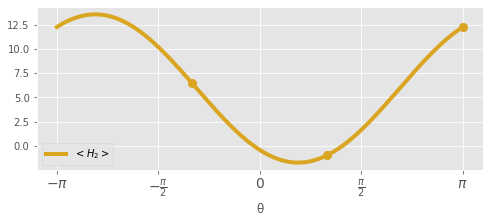
\includegraphics[width=.34\paperwidth]{Figures/h2_optimization} \\
				\small{$32$ samples $\rightarrow$ $3$ samples}
			\end{center}

			\columnbreak

			\begin{center}
				\texttt{ \small
					GROUND-STATE ENERGY (H3): \\
					Minimum \underline{'E3 = -2.0509 (MeV)'} \\
					'[theta, eta] = [0.2688, 0.3631] (rad)' \\
					>> ERROR = 0.2\% } \\
				\smallskip
				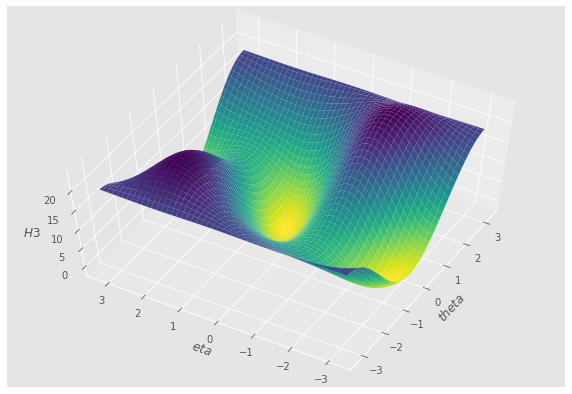
\includegraphics[width=.34\paperwidth]{Figures/h3_optimization} \\
				\small{$400$ samples $\rightarrow$ $25$ samples}
			\end{center}

		\end{multicols}

	\end{frame}

%%%%%%%%%%%%%%%%%%%%%%%%%%%%%%%%%%%%%%%%%%%%

	\subsection{Future Work}

	\begin{frame}{Future Work}

		There are some different paths we can go down from here:

		\begin{itemize}
			\item Study the impact of \textbf{noise} on this new method
			\item Determine the \textbf{range of cases} which benefit form this new approach and its applicability
			\item Extrapolate this entire procedure to the study of \textbf{new and more interesting problems}
		\end{itemize}

	\end{frame}

%%%%%%%%%%%%%%%%%%%%%%%%%%%%%%%%%%%%%%%%%%%%
%%%%%%%%%%       REFERENCES       %%%%%%%%%%
%%%%%%%%%%%%%%%%%%%%%%%%%%%%%%%%%%%%%%%%%%%%

\section{References}
%	\begin{frame}[allowframebreaks]{References}
	\begin{frame}{References}

		\begin{thebibliography}{9}

			\setbeamertemplate{bibliography item}[article]
			\bibitem{dumitrescu} \textbf{Dumitrescu, E.F. (et al.)} \emph{Cloud Quantum Computing of an Atomic Nucleus}

			\setbeamertemplate{bibliography item}[article]
			\bibitem{lee} \textbf{Lee, J. (et al.)} \emph{Generalized Unitary Coupled Cluster Wavefunctionsfor Quantum Computation}

			\setbeamertemplate{bibliography item}[article]
			\bibitem{peruzzo} \textbf{Peruzzo, A. (et al.)} \emph{A variational eigenvalue solver on a photonic quantum processor}

			\setbeamertemplate{bibliography item}[article]
			\bibitem{mcmclean} \textbf{McMClean, J.R.} \emph{The theory of variational hybrid quantum-classical algorithms}

			\setbeamertemplate{bibliography item}[article]
			\bibitem{shannon} \textbf{Shannon, C.E.} \emph{Communication in the Presence of Noise}

			\setbeamertemplate{bibliography item}[book]
			\bibitem{nielsen} \textbf{Nielsen, M.A. \& Chuang, I.L.} \emph{Quantum Computation and Quantum Information}

		\end{thebibliography}

		\vspace{20pt}
		\begin{small}
		\begin{center}{
		\color{gray}
			\emph{"The only thing demonstrated by an impossibility proof is a lack of imagination."} \\
			\textbf{– John Stewart Bell –} }
		\end{center}
		\end{small}
	\end{frame}

\FinalFrame

\end{document}
